\documentclass[12pt,titlepage,a4paper]{report}
% Texte
\usepackage[utf8]{inputenc}
\usepackage[T1]{fontenc}
\usepackage[french]{babel}
\usepackage{lmodern}
\usepackage{float}
\usepackage{enumitem}
\usepackage{minted}
% Pour les checkmarks
\usepackage{pifont}
\usepackage{amssymb}
% Pour des \hline en gras
\usepackage{makecell}
% Numéroter les chapitres à partir de chaque début de partie
\makeatletter\@addtoreset{chapter}{part}\makeatother

% Mise en page
\usepackage{url}
\usepackage[top=2.1cm,bottom=2cm,left=3cm,right=3cm]{geometry}
\usepackage{hyperref}
\hypersetup{
    colorlinks=false,
    pdfborder={0 0 0},
}
\usepackage{multirow}

% TOC
\usepackage[french]{minitoc}
\setcounter{tocdepth}{2}
\setcounter{minitocdepth}{2}
\setlength{\mtcindent}{0pt}

% Maths
\usepackage{amsmath}
\usepackage{amssymb}
\newcommand{\reels}{\mathbb{R}}

% Images
\usepackage{float}
\usepackage{wrapfig}
\usepackage{graphicx}
% Pour inclure des pages PDF
\usepackage[final]{pdfpages}

% Couverture
\usepackage{templateINSA}
\initINSA

\title{Classification de nuages de points}
\author{Manon \bsc{Ansart}\\ Aurélien \bsc{Massiot}}

\renewcommand\soustitre{Rapport de projet}
\renewcommand\infoBig{Projet d'Approfondissement et d'Ouverture}
\renewcommand\infoSmall{ASI4 2014-2015}
\newcommand{\code}[1]{\texttt{#1}}
\newcommand{\hlineGras}{\Xhline{2\arrayrulewidth}}

\def\changemargin#1#2{\list{}{\rightmargin#2\leftmargin#1}\item[]}
\let\endchangemargin=\endlist

\begin{document}
	\titleINSA{15}{images/objet3D2.jpg}{0}{0}{227}{}{\textcolor{white}{}}

	\dominitoc
	\tableofcontents

	\chapter{Introduction}
		Aujourd'hui, les technologies et l'intelligence artificielle ne cessent de progresser. Les appareils que nous utilisons dans la vie de tous les jours, tels que les téléphones portables et appareils électroménagers, sont de plus en plus performants mais aussi plus intelligents. C'est aussi le cas de nos véhicules de transport, comme les voitures qui peuvent se garer automatiquement, et parfois même détecter des "objets" tels que des piétons.\\

Les voitures grand public sont donc en grande majorité équipées de différents capteurs. Les capteurs CMOS (complementary metal oxide semiconductor) et CCD (charge coupled device) sont particulièrement utilisés pour ces applications. Les CCD, créés en 1969, sont composés d'une série de condensateur semi-conducteurs chargés par la lumière selon son intensité. Les charges sont ensuite transformées en tension pour être mesurer. Ces capteurs, plus utilisés à l'origine, étaient moins sensibles au bruit et avaient une sortie de bonne qualité. Ils ont petit à petit été remplacés par les capteurs CMOS, créés au début des années 90. Ces capteurs sont moins chers et plus simples à utiliser, ce qui explique leur succès. Ces capteurs sont utilisés sur beaucoup de voitures, par exemple pour aider à la conduite de nuit, ou surveiller la somnolence du conducteur.\\

Les voitures orientées recherche ont davantage d'intelligence et de précision ; dès 2005, la voiture "Alice" de la Team Caltech pouvait rouler 300 miles en autonomie et en évitant les obstacles en un environnement inconnu, dans le cadre du DARPA Grand Challenge dans le désert des Mojaves. La voiture "Junior", de Stanford University, est capable de naviguer dans un environnement urbain en autonomie. Elle est capable de sélectionner ses propres routes, percevoir le traffic alentour, et effectuer des manœuvres telles que des changements de voies, des demi-tours et des stationnements. Elle a ainsi obtenu la seconde place du DARPA Urban Challenge de 2007 qui se déroulait cette fois en milieu urbain. La plateforme PACPUS du laboratoire Heudiasyc, rattachée à l'Université de Technologie de Compiègne, est composée de plusieurs véhicules expérimentaux qui permettent de tester des aides à la conduite automobile et des fonctions ADAS (Advanced Driver Assistance Systems). Ces véhicules sont équipés de capteurs et logiciels permettant des applications comme la localisation précise (trajectométrie de précision centimétrique), la perception de l'environnement et du conducteur grâce à des télémètres laser, caméras numériques et radars, ou encore des mesures temps réel de la dynamique du véhicule (dérive, forces sur les roues).\\

Justement, pouvoir détecter des objets susceptibles d'entrer en collision avec son véhicule est un progrès considérable pour la sécurité de chacun. Savoir de plus quel est cet objet, afin d'adopter un comportement propre à chacun, est encore plus intéressant. Nous pouvons par exemple demander au véhicule de ralentir lorsqu'un cycliste ou un piéton est à proximité, et continuer sa route si l'objet identifié est un arbre, puisque celui-ci ne peut a priori pas bouger.\\

Nous pouvons dès lors nous demander comment une telle classification d'objets pourrait être réalisée ; comment capturer des données et les utiliser à bon escient afin d'en extraire des caractéristiques propres à chaque objet ?\\

Nous allons donc étudier dans un premier temps les attributs nous permettant de réaliser la classification. Dans un deuxième temps, nous allons décrire les classifieurs utilisés après avoir extraits les attributs propres à chaque classe d'objet. Enfin, nous allons parler de la librairie C++ PointClouds, qui peut être intéressante pour traiter des images 3D.\\
        \chapter{Jeu de données}
		\section{Extraction des données}

	Les données sont extraites à partir de ROS. Il s'agit d'un outil qui sert à traiter les .tm, qui sont des vidéos en 3D, pour en extraire des nuages de points au format pcd. Ici, les vidéos que nous avons sont filmées depuis un véhicule dans une zone urbaine.\\

	Vu qu’il y a des erreurs dans la compilation du C++ pour lancer ROS, M. Guerrero nous a fourni directement les archives contenant les pcd.\\

\section{Description des données}

	Les données que nous avons sont une multitude imagettes (frames) de chaque classe. Ce sont des sortes de captures d'écran d'une vidéo à un instant donné, mais en trois dimensions.\\

	Au total, nous avons les classes suivantes : 
	% à compléter classe + nombre d'images de la classe

	Soit$ X_{i}$ la ième imagette, on a :

	$  X_{i} \in \reels^{n_{i}*4} $, avec 50 $\leq n_{i} \leq 300$
	En effet, chaque imagette a ses coordonnées x, y, z et une valeur d'intensité. \\ 

\section{Jeu de données lomita}

	Ce jeu de données contient 75817 imagettes réparties dans 155 séquences de 5 classes différentes : background, bicyclist, car, pedestrian et unlabeled. On remarquera cependant que les données ne sont pas également réparties entre ces 5 classes : il y a 105 background, 5 bicyclist, 20 car, 9 pedestrian et 16 unlabeled.
	\chapter{Choix des attributs}
		Afin de mettre en place nos classifieurs pour identifier les nuages de points 3D, nous avons tout d'abord dû extraire plusieurs métriques nous permettant de représenter nos images de points. Nous prenions pour cela en entrée un fichier par nuage de points, comportant pour chaque point ses coordonnées (x, y et z) et son intensité. Voici en figure \ref{fig:nuage_de_points} un exemple de nuage de points représentant un cycliste :

	\begin{figure}[H]
		\centering
		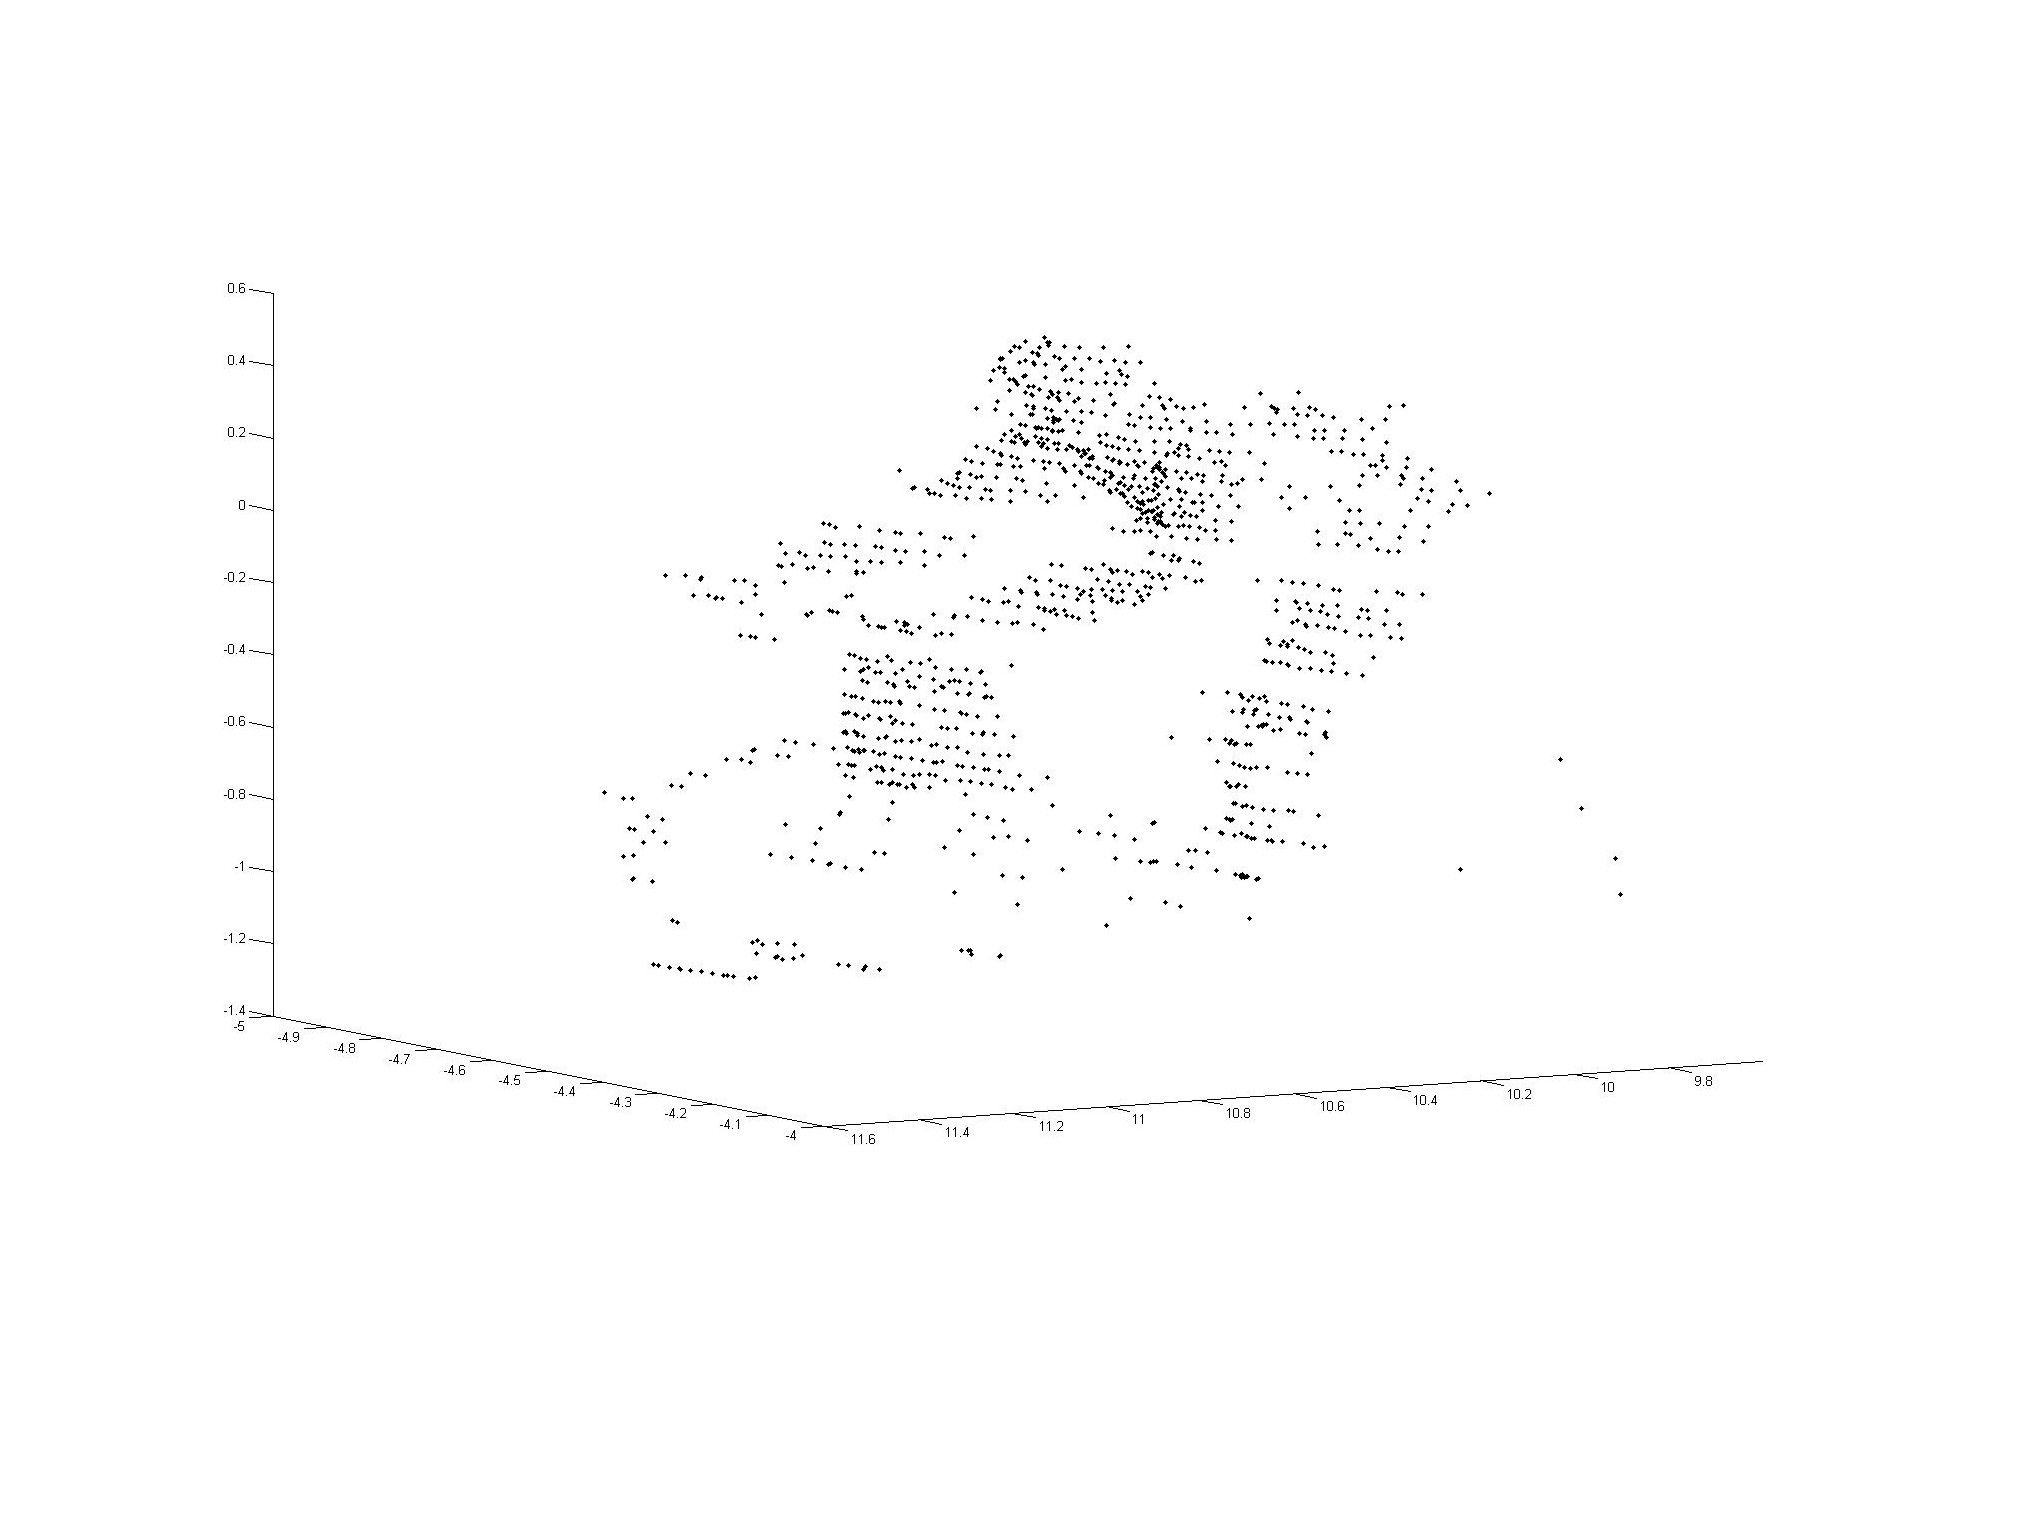
\includegraphics[scale=0.25]{images/objet3D2.jpg}
		\caption{Exemple de \emph{nuage de points}}
		\label{fig:nuage_de_points}
	\end{figure}

\section{Attributs utilisés}
	\subsection{Métriques statistiques basiques}
		Dans un premier temps, nous avons extrait des métriques statistiques très simples basées sur l'intensité des points. Nous avons pour chaque nuage de points calculé la moyenne, la variance, le minimum et le maximum des intensités.\\

		En effet, ces valeurs changent selon les classes. On peut le voir dans le tableau suivant, présentant les moyennes des quatre attributs sur des nuages de points de type voitures et background :\\

		\begin{center}
			\begin{tabular}{|l||c|c|c|c|}
			  \hline
			  & Minimum & Maximum & Moyenne & Variance \\
			  \hline
			  Voitures & 34.5 & 249 & 120 & 3500 \\
			  Background & 48.7 & 196 & 125 & 1548 \\
			  \hline
			\end{tabular}
		\end{center}


		Cela nous montre que ces attributs peuvent présenter des différences significatives selon les classe, il est donc intéresssant de prendre en compte ces métriques pour la classification.

	\subsection{Bounding-box}
		La \emph{bounding-box} permet de connaître la forme de l'objet en 3D pour distinguer des objets de catégorie différentes.

		\begin{figure}[H]
			\centering
			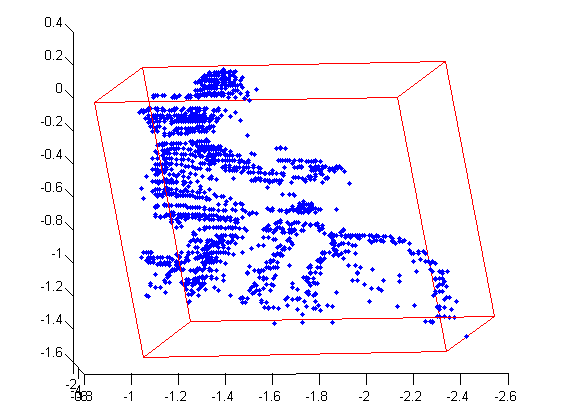
\includegraphics[scale=0.6]{images/bounding_box_cyclist_2.png}
			\caption{Exemple de \emph{bounding-box} sur un cycliste}
			\label{fig:image}
		\end{figure}
		% Source : http://www.mathworks.com/matlabcentral/fileexchange/screenshots/2122/original.jpg

		La \emph{bounding-box} représente l'amplitude du nuage de points selon les trois dimensions. Pour chaque dimension, nous aurons donc un attribut qui correspond à la différence entre le maximum de cette coordonnée et le minimum de cette coordonnée, pour chaque nuage de points.\\

		Afin de pouvoir calculer la \emph{bounding-box}, nous avons dû "redresser" le nuage de points selon l' axe $z$, en considérant que le terrain est plat et qu'il n'y a donc pas besoin de redresser l'image selon $x$ et $y$).
		Nous avons donc calculé l'angle $\theta$ de la rotation, grâce à la formule:

		\[ tan(2 \theta) = 2 * \frac{\bar{x}\bar{y}}{\bar{x}^2 - \bar{y}^2} \]
		\[ \theta = \frac{1}{2} * arctan(2 \frac{\bar{x}\bar{y}}{\bar{x}^2 - \bar{y}^2}) \]

		avec \[ \bar{x} = \frac{1}{n} * \sum_{i =1}^n{x_i} \]
		\[ \bar{y} = \frac{1}{n} * \sum_{i =1}^n{y_i} \]

		Une fois que nous avons trouvé l'angle de rotation, il faut appliquer la rotation au nuage de points. Pour cela on construit la matrice $R_z$ telle que :

		\[\begin{bmatrix}
		   cos(\theta) & -sin(\theta) & 0 \\
		sin(\theta) & cos(\theta) & 0 \\
		0 & 0 & 1
		\end{bmatrix}\]

		On calcule ensuite le nouveau nuage de point redressé avec la formule:
		\[ P_T = R_z * P_0\]
		où $P_0$ est le nuage de points d'origine. \\

		Nous appliquons ensuite une translation à l'origine sur le nuage de point redressé pour le centrer. On peut maintenant calculer les 3 attributs de la \emph{bounding-box} sur ce nouveau nuage de points.


	\subsection{Scatter-ness, linear-ness et surface-ness}
		D'autres attributs intéressants à étudier dans le cadre de la reconnaissance d'objets 3D sont la \emph{scatter-ness}, la \emph{linear-ness} et la \emph{surface-ness}, qui traduisent la forme de l'objet.

		Pour les calculer, on calcule tout d'abord la matrice de covariance des coordonnées des points, puis on calcule les valeurs propres $\lambda_0$, $\lambda_1$ et $\lambda_2$ de la matrice de covariance. \\

		On s’intéresse ensuite à la différence entre ces valeurs :
		\begin{itemize}
			\item Si ces trois valeurs sont similaires ($\lambda_0 \approx \lambda_1 \approx \lambda_2$), les points sont répartis de manière égale selon les trois dimensions, comme pour une sphère. On dit qu'ils sont dispersés et on parle de \emph{scatter-ness}.
			\item Si au contraire une valeur est beaucoup plus grande que les deux autres ($\lambda_0 \gg \lambda_1 \approx \lambda_2$), cela signifie que les points sont principalement répartis sur une seule dimension, ils forment une sorte de ligne. On parle alors de \emph{linear-ness}.
			\item Si une valeur est beaucoup plus petite que les deux autres ($\lambda_0 \approx \lambda_1 \gg \lambda_2$), cela signifie que les points sont répartis sur deux dimensions, et forment quasiment une surface. On parle alors de \emph{surface-ness}.\\
		\end{itemize}

		Nous allons donc nous intéresser aux attributs suivants :
		\begin{itemize}
			\item $\lambda_0$, qui représente la \emph{scatter-ness};
			\item $\lambda_0 - \lambda_1$, qui représente la \emph{linear-ness};
			\item $\lambda_1 - \lambda_2$, qui représente la \emph{surface-ness};
		\end{itemize}

\section{Attribut étudié : les spin-images}

	La spin image est l’image du nuage 3D prise en un point, perpendiculairement à la normale en ce point (donc selon le plan tangent). Le but est de prendre est de prendre les meilleures spin images pour chaque nuage de point car c’est sur ces images 2D que nous pouvons réaliser une classification.




\section{Autres attributs possibles}

        \chapter{Classification}
		\section{Description des classifieurs utilisés}

	Il nous était possible d'utiliser deux sortes d'apprentissage sur nos données. L'apprentissage non-supervisé apprend uniquement à partir des attributs, sans tenir compte des labels. Cela permet par exemple de faire du clustering pour regrouper les données en différentes classes. Nous avons appliqué cette méthode d'apprentissage en utilisant l'algorithme des k-moyennes sur nos données.\\

	L'apprentissage supervisé apprend en se basant sur les attributs mais en utilisant également les labels que nous connaissons. Cette technique d'apprentissage paraît donc plus adaptée dans notre cas. Différentes méthodes existent, nous avons choisis de nous concentrer sur les SVM (\emph{Support Vector Machines} ou séparateurs à vaste marge) pour réaliser notre classification en apprentissage supervisé. Ils sont souvent utilisés pour résoudre des problèmes de discrimination, c'est-à-dire savoir à quelle classe appartient un échantillon, et c'est exactement le problème auquel nous sommes confrontés. Le SVM va chercher à tracer une limite entre les classes des données d'apprentissage en maximisant la marge entre cette limite et chaque classe. Les classes de nouvelles données seront ensuite attribuées selon le côté du quel se trouvent les nouvelles données. La limite entre les classes peut-être en ligne droite, dans le cas d'un SVM linéaire, ou plus compliquée dans le cas d'un SVM avec noyau.\\

	Dans un premier temps nous avons travaillé sur deux classes, ce qui est le problème le plus simple à résoudre avec des SVM. Nous avons pour cela réalisé deux SVM, un SVM linéaire et un SVM gaussien. Nous avons effectué de la validation croisée afin d'identifier les hyper-paramètres (C pour le SVM linéaire, et C et sigma pour le SVM gaussien).

	Dans un second temps nous avons travaillé sur un jeu de données contenant 4 classes et des données \emph{unlabeled} représentant une cinquième classe. Les données unlabeled ont été retirées de l'ensemble de l'apprentissage car elle pouvait correspondre à n'importe quelle classe et donc perturber le SVM.
	Nous avons ensuite utilisé deux méthodes permettant de faire de la classification avec plus de deux classes :

	\begin{itemize}
	\item La méthode \emph{one-versus-all} consiste à construire M classifieurs binaires en attribuant le label 1 aux échantillons de l'une des classes et le label -1 à toutes les autres. En phase de test, la classe est determinées grâce à un vote à la majorité entre les différents SVM.
	\item La méthode \emph{one-versus-one} consiste à construire $\frac{M(M-1)}{2}$ classifieurs binaires en confrontant chacune des $M$ classes. En phase de test, l'échantillon à classer est analysé par chaque classifieur et un vote majoritaire permet de déterminer sa classe.\\
	\end{itemize}


\section{Données et pré-traitement}
\subsection{Extraction des données}

	Les données sont extraites à partir de ROS. Il s'agit d'un outil qui sert à traiter les \texttt{.tm}, qui sont des vidéos en 3D, pour en extraire des nuages de points au format pcd. Ici, les vidéos que nous avons sont filmées depuis un véhicule dans une zone urbaine.\\

	Vu qu’il y a des erreurs dans la compilation du C++ pour lancer ROS, M. Guerrero nous a fourni directement les archives contenant les pcd.\\

\subsection{Format des données}

	Les données que nous avons sont une multitude d'imagettes (frames) de chaque classe. Ce sont des sortes de captures d'écran d'une vidéo à un instant donné, mais en trois dimensions.\\

	Soit$ X_{i}$ la ième imagette, on a :

	$  X_{i} \in \reels^{n_{i}*4} $, avec 50 $\leq n_{i} \leq 300$
	En effet, chaque imagette a ses coordonnées $x$, $y$, $z$ et une valeur d'intensité. \\

\subsection{Jeu de données dish area}

	Ce jeu de données contient 30242 imagettes réparties dans 91 séquences de 2 classes différentes : background et car. On remarquera cependant que les données ne sont pas également réparties entre ces classes : il y a 26715 imagettes de la classe background et 3527 de la classe car.

\subsection{Jeu de données lomita}

	Ce jeu de données contient 75817 imagettes réparties dans 155 séquences de 5 classes différentes : background, bicyclist, car, pedestrian et unlabeled. On remarquera cependant que les données ne sont pas également réparties entre ces 5 classes : il y a 60103 imagettes de classe background, 958 bicyclist, 5937 car, 1831 pedestrian et 6984 unlabeled. \\

	La classe unlabeled n'est pas une classe en soit, elle regroupe les imagettes n'ayant pas pu être classées dans une des 4 autres classes. Ces données ont donc été supprimées du jeu de données car elles auraient pu fausser l'apprentissage. \\

	Nous avons également ré-équilibré les classes en utilisant seulement une partie de la classe background afin que la différence d'effectif entre cette classe et les autres ne soit pas trop importante. Nous avons donc pris aléatoirement 7000 données de la classe background sur les 60103 présente à l'origine, ce qui correspond à une sélection de 11,65\%. Ce changement a nettement amélioré nos résultats. Nos machines n'étant pas assez puissantes, nous n'avons pas pu faire tourner nos propres algorithmes sur la totalité des données sans retirer des données de la classe background. Nous les avons cependant exécutés sur une partie des données (1722 observations) non ré-équilibrées et avons conservé ces résultats à titre de comparaison. \\


\section{Résultats obtenus}


	\subsection{Classification sur deux classes (dish area)}
		\subsubsection{K-moyennes}
			Nous avons utilisé l'algorithme kmeans de matlab pour former des clusters et les comparer avec les classes connues. Nous obtenons un taux d'erreur de 8.71\%, ce qui est un bon résultat pour un algorithme non-supervisé. Notre matrice de confusion est la suivante :

			\begin{center}
				\begin{tabular}{|l||c|c|}
				  \hline
				  \backslashbox{Vérité}{Prédiction}& background & car \\
				  \hline
				  background & 25054 & 1661 \\
				  \hline
				  car & 974 & 2553 \\
				  \hline
				\end{tabular}
			\end{center}

			On constate que les erreurs sont plutôt bien réparties, c'est-à-dire qu'il n'y a pas plus d'erreur pour une classe pour une autre, ce qui était un risque étant donné que nos classes n'ont pas le même effectif.

		\subsubsection{SVM linéaire}
			Nous avons créé un SVM linéaire en effectuant de la validation croisée pour le paramètre C. Nous avons pour cela utilisé la fonction monqp de la toolbox SVM-KM. En l’exécutant sur la totalité des données nous obtenons un taux d'erreur de A changer !!!\%. Notre matrice de confusion est la suivante :
			\begin{center}
				\begin{tabular}{|l||c|c|}
				  \hline
				  \backslashbox{Vérité}{Prédiction}& background & car \\
				  \hline
				  background & A changer !!! & A changer !!! \\
				  \hline
				  car & A changer !!! & A changer !!! \\
				  \hline
				\end{tabular}
			\end{center}

			COMMENTAIRE !
		\subsubsection{SVM gaussien}
			Nous avons créé un SVM gaussien en effectuant de la validation croisée pour le paramètre C et le paramètre sigma. Pour le paramètre C nous avons choisi d'utiliser une valeur différente pour les deux classes. Nous avons donc effectuer la validation séparément pour ces deux valeurs de C. En l’exécutant sur la totalité des données nous obtenons un taux d'erreur de A changer !!!\%. Notre matrice de confusion est la suivante :
			\begin{center}
				\begin{tabular}{|l||c|c|}
				  \hline
				  \backslashbox{Vérité}{Prédiction}& background & car \\
				  \hline
				  background & A changer !!! & A changer !!! \\
				  \hline
				  car & A changer !!! & A changer !!! \\
				  \hline
				\end{tabular}
			\end{center}

			COMMENTAIRE !

	\subsection{Classification sur quatre classes (lomita)}

		\subsubsection{K-moyennes}
			Nous avons utilisé l'algorithme kmeans de matlab pour former des clusters et les comparer avec les classes connues. Cet algorithme étant très optimisé, c'est le seul que nous avons pu exécuter sur la totalité de nos données. Nous obtenons un taux d'erreur de 23.9\%. Ce taux est très élevé. En effet, la classe background étant sur-représentée, un algorithme prédisant tout le temps la classe background aurait de meilleures performances (12.7 \%).

			\begin{center}
				\begin{tabular}{|l||c|c|c|c|}
				  \hline
				  \backslashbox{Vérité}{Prédiction}& background & bicyclist & car & pedestrian \\
				  \hline
				  background & 51258 & 8845 & 0 & 0 \\
				  \hline
				  bicyclist & 78 & 880 & 0 & 0 \\
				   \hline
				  car & 1964 & 3973 & 0 & 0 \\
				   \hline
				  pedestrian & 708 & 1123 & 0 & 0 \\
				  \hline
				\end{tabular}
			\end{center}

			On remarque que les résultats sur les deux premières classes sont convenables mais les deux dernières classes ne sont jamais prédites.

		\subsubsection{SVM one-versus-one}

			Nous avons mis en place notre propre SVM One versus one. Cette méthode met en place plusieurs SVM comparant les classes une à une, puis un vote à la majorité nous permet de prédire la classe pour une nouvelle donnée. Cette méthode étant coûteuse en temps, nous avons choisi d'utiliser uniquement des SVMs linéaire. Nous avons retenu une version qui effectue la validation croisée du C sur l'ensemble du SVM multi-classe, le même C est donc retenu pour tous les SVM. Nous avons également créé une autre version, pour laquelle la validation croisée est effectuée sur chaque SVM individuellement, qui obtient un taux d'erreur légèrement meilleur mais pour un temps de calcul plus long. Cette version n'est pas la version retenue à cause des temps de calcul, elle ne sera donc pas commentée ici mais elle est disponible dans le dossier.
			
			\paragraph{Données non rééquilibrées :}
				Nous obtenons 4.4 \% d'erreurs sur le petit jeu de données. Notre matrice de confusion est la suivante :

				\begin{center}
					\begin{tabular}{|l||c|c|c|c|}
					  \hline
					  \backslashbox{Vérité}{Prédiction}& background & bicyclist & car & pedestrian \\
					  \hline
					  background & 372 & 3 & 0 & 0 \\
					  \hline
					  bicyclist & 4 & 2 & 0 & 0 \\
					   \hline
					  car & 1 & 0 & 36 & 0 \\
					   \hline
					  pedestrian & 10 & 1 & 0 & 0 \\
					  \hline
					\end{tabular}
				\end{center}

				On remarque que, même si notre taux d'erreur est bon, les erreurs ne sont pas bien réparties entre les classes. Notre SVM ne prédit jamais la bonne classe pour les imagettes de classe pedestrian et les résultats sont également faibles pour la classe bicyclist.

			\paragraph{Données rééquilibrées :}
				Nous obtenons 0 \% d'erreurs sur le jeu de données rééquilibré, ce qui est très surprenant. Notre matrice de confusion est la suivante :

				\begin{center}
					\begin{tabular}{|l||c|c|c|c|}
					  \hline
					  \backslashbox{Vérité}{Prédiction}& background & bicyclist & car & pedestrian \\
					  \hline
					  background & 1750 & 0 & 0 & 0 \\
					  \hline
					  bicyclist & 0 & 239 & 0 & 0 \\
					   \hline
					  car & 0 & 0 & 1484 & 0 \\
					   \hline
					  pedestrian & 0 & 0 & 0 & 457 \\
					  \hline
					\end{tabular}
				\end{center}
			\vspace{10 mm}

		\subsubsection{SVM one-versus-all}
			Nous avons mis en place un SVM one versus all en utilisant les fonction svmclass et svmval, permettant respectivement d’entraîner les SVMs et d'obtenir des prédictions. Grâce à ces fonctions nous avons créé des SVMs comparant chaque classe aux autres, puis la classe des nouvelles données étaient prédites grâce à un vote à la majorité. Nous n'avons pas ajouté de validation croisée sur ce SVM car cela était trop coûteux en temps. Nous avons utilisé des SVM avec noyau gaussien.

			\paragraph{Données non rééquilibrées :}
				Nous avons obtenu un taux d'erreurs de 4.65 \% sur le petit jeu de données. La matrice de confusion est la suivante :
				\begin{center}
					\begin{tabular}{|l||c|c|c|c|}
					  \hline
					  \backslashbox{Vérité}{Prédiction}& background & bicyclist & car & pedestrian \\
					  \hline
					  background & 595 & 1 & 0 & 5 \\
					  \hline
					  bicyclist & 4 & 1 & 0 & 4 \\
					   \hline
					  car & 4 & 0 & 55 & 0 \\
					   \hline
					  pedestrian & 14 & 0 & 0 & 4 \\
					  \hline
					\end{tabular}
				\end{center}

				On remarque que les résultats sont plutôt bons pour les classes background et car mais moins pour les deux autres, qui sont moins représentées.

			\paragraph{Données non rééquilibrées :}
				Nous avons obtenu un taux d'erreurs de 0.175 \%. La matrice de confusion est la suivante :
				\begin{center}
					\begin{tabular}{|l||c|c|c|c|}
					  \hline
					  \backslashbox{Vérité}{Prédiction}& background & bicyclist & car & pedestrian \\
					  \hline
					  background & 2800 & 0 & 0 & 0 \\
					  \hline
					  bicyclist & 0 & 383 & 0 & 0 \\
					   \hline
					  car & 1 & 4 & 2369 & 0 \\
					   \hline
					  pedestrian & 5 & 0 & 1 & 726 \\
					  \hline
					\end{tabular}
				\end{center}

				Ces résultats sont vraiment bons.


	\subsection{Commentaire des résultats}
		RAJOUTER UNE CONLUSION SUR LES 2 CLASSES ?

		Nous avons pu voir que, si la classification non-supervisée donne des résultats convenables sur deux classes, les résultats deviennent vraiment faibles pour la classification multi-classe.

		Les SVM obtiennent de bons résultats. Lorsque les données ne sont pas rééquilibrées il y a des erreurs importantes sur les classes les moins représentées (bicyclist et pedestrian). Les méthodes que nous avons vues ne permettent pas de classifier convenablement ces classes en gardant les données telles quelles. Ces erreurs disparaissent cependant lorsque nous diminuons le nombre d'observations pour la classe background. Les erreurs des autres classes diminuent considérablement sans que cela ait de conséquences sur la classification de la classe background, ce qui entraîne une diminution significative de l'erreur. Les résultats obtenus, avec des erreurs inférieures à 0.2 \% ou nulles, sont remarquables.

		Ces résultats sont toute fois à nuancer puisque des tirages aléatoires sont réalisés pour rééquilibrer la classe background et pour construire les ensemble d'apprentissage, de validation et de test. Des tirages différents pourraient donc amener à des résultats légèrement différents. Il pourrait être intéressant d'exécuter les algorithmes plusieurs fois avec des tirages différents afin de calculer les différentes erreurs et d'en faire la moyenne. Cela serait cependant coûteux en temps, à raison d'une heure par exécution.


        \chapter{Utilisation de PCL}
		PCL, ou Point Cloud Library, est une librairie C++ open source utilisée pour les traitements d'images 2D/3D et de nuages de points.\\

\section{Utilisation de PCL}

	Comme dit précédemment, le dataset original est dans un format de fichier vidéo tm. Les données ont donc été extraites en utilisant une application basée sur ROS, puis exportées en format PCD. Les fichiers PCD sont des nuages de points 3D. Pour traiter ces données, nous avons donc utilisé la bibliothèque PCL en C++, qui est une plateforme utilisée dans des applications robotiques, développée depuis 2010 et est toujours en développement. Elle regroupe de nombreuses techniques de traitement d'images comme des nouvelles méthodes d'extraction des attributs et de "keypoints", de classification, de reconstruction de surface, de reconnaissance de forme, ou encore de filtrage de bruit.

\section{Formation sur PCL}

	Nous nous sommes donc formés sur PCL. La première chose à faire était de visualiser nos données ; nous avons pour cela utilisé \emph{PCLVisualizer}, proposé dans le tutoriel \url{http://pointclouds.org/documentation/tutorials/pcl_visualizer.php#pcl-visualizer}. Toutefois, nous avons dû centrer nos données manuellement par rapport aux axes afin d'obtenir une visualisation correcte.\\

	Dans le dossier essai\_segmentation, nous avons testé une méthode de segmentation plane afin de mieux appréhender la librairie PointClouds.\\
	Des points sont d'abord générés de façon à former un plan, et d'autres sont volontairement placés à l'écart. Le programme cherche ensuite les points qui forment un plan, et calcule ses paramètres.\\

	De même, dans le dossier essai\_segmentation\_2, nous avons testé une méthode de segmentation par croissance de régions. A noter cependant que cela ne fonctionne pas avec nos fichiers .pcd (core dump), nous avons dû utiliser le fichiers .pcd donné dans le tutoriel associé.\\

	Nous avons aussi essayé d'extraire des spin images depuis nos données, en utilisant la classe SpinImage de PCL ; mais les méthodes implémentées ne permettent pas de calculer des spin images sur des nuages dont le nombre de points est faible, comme les nôtres.\\

\section{Utilisation de Matlab}

	Nous avons finalement utilisé Matlab plutôt que PCL, pour plusieurs raisons. La première est qu'il n'y a pas autant de méthodes de classification (non supervisées ou supervisées) déjà opérationnelles sur PCL par rapport à Matlab. Il y a quelques fonctions de clustering en PCL mais il s'agit d'apprentissage non-supervisé alors que nous avons un problème d'apprentissage supervisé : nous connaissons déjà les classes dans lesquelles nous voulons classifier nos objets.\\

	De plus, le temps de développement sur PCL est supérieur à Matlab puisque nous connaissons beaucoup mieux le langue associé à Matlab comparé au C++, puisque c'est avec Matlab que nous avons implémentés nos algorithmes en cours de Fouille de Données. \\

	PCL est plus performant pour effectuer des calculs en temps réel par rapport à Matlab, mais étant donné que nos calculs se font offline, nous avons privilégié Matlab. \\

	Finalement, PCL aurait pu nous servir pour extraire des caractéristiques de nos nuages de points, mais nous nous sommes rendus compte que cette librairie permettait surtout d'effectuer du traitement sur des images 3D ayant des milliers de points et en XYZRGB.\\


	\chapter{Conclusion}
		Finalement, nous avons pu constater que la classification d'objets, aujourd'hui de plus en plus présente notamment dans les véhicules intelligents, n'est pas si compliquée que cela. En effet, en extrayant des nuages de points à partir de vidéos, puis en calculant de simples attributs sur ces nuages, nous avons pu classifier des objets tels que des piétons ou des arbres dans leurs classes respectives. Bien évidemment, pour améliorer encore nos résultats, nous pourrions ajouter beaucoup d'autres attributs tels que des spin images ou des bounding boxes exactes par exemple, en entrée dans notre classifieur. Nous pourrions aussi améliorer les choix des hyper-paramètres dans nos SVM (Support Vector Machines). Enfin, nous pourrions essayer d'autres classifieurs ; les forêts aléatoires (Random Forests), notamment, ou des techniques de boosting comme Adaboost pourraient être une piste de comparaison.\\

Même si nous avons perdu du temps à essayer de manipuler la librairie Pointclouds, nous avons pu apprendre un peu à la manipuler, et nous la connaissons désormais un peu afin éventuellement de l'utiliser dans d'autres projets plus adéquats par rapport aux capacités de cette librairie.\\

Enfin, nous sommes satisfaits d'avoir pu appliquer nos connaissances théoriques d'apprentissage automatique sur un problème concret. Comme dit précédemment, la classification d'objets va se rendre de plus en plus indispensable dans des dispositifs qui ont besoin d'informations en temps réel, et de réagir en conséquence ; grâce à cela, peut-être aurons nous bientôt des robots faisant la cuisine en choisissant les ingrédients grâce à des caméras?\\
    \chapter{Sources}
        \textbf{Bounding box} :
\begin{itemize}
	\item http://en.wikipedia.org/wiki/Minimum\_bounding\_box
	\item http://fr.mathworks.com/help/images/ref/regionprops.html
\end{itemize}

\textbf{Matlab} : 
\begin{itemize}
	\item http://fr.mathworks.com
\end{itemize}

\textbf{Pointclouds} : 
\begin{itemize}
	\item http://pointclouds.org/
	\item http://en.wikipedia.org/wiki/Point\_cloud
\end{itemize}

\textbf{Spin images} :
\begin{itemize}
	\item http://homepages.inf.ed.ac.uk/rbf/CVonline/LOCAL\_COPIES/AV0910/SpinImages.pdf
\end{itemize}

\textbf{Support Vector Machines - généralités} : 
\begin{itemize}
	\item http://en.wikipedia.org/wiki/Support\_vector\_machine
	\item https://www.lri.fr/~antoine/Courses/Master-ISI/ISI-10/Tr-cours-SVM\_2014\_2x2.pdf
\end{itemize}

\textbf{Support Vector Machines - classification d'objets} :
\begin{itemize}
	\item http://www.cs.dartmouth.edu/~afra/courses/44/w09/project/report/gu-song-report.pdf
	\item http://olivier.chapelle.cc/pub/intern98.pdf
\end{itemize}

%http://www.osa-opn.org/home/articles/volume_23/july_august/features/vision_sensors_in_automobiles_an_indian_perspectiv/#.VV2sW3Xtmko
%http://www.usinenouvelle.com/article/objectif-zero-conducteur.N147173

    % Bibliographie
	\nocite{*} %pour citer les sources sans mettre de référence dans le texte
	\bibliographystyle{abbrv} %classé par ordre alphabétique et certains mots abrégés
	\bibliography{textes/bibli}
\end{document}
